
\documentclass[a4paper,11pt]{article}
\usepackage{graphicx}

\title{Features for the GSoC 2010 Project:\\
       3D Visualization for Interplanetary Trajectories}
\author{
      Edgar Sim\'{o} Serra \\
      Mentored by Chit-Hong Yam and Dario Izzo 
}
\date{\today}

\begin{document}
\maketitle

\begin{abstract}
Future intended feature set for the 3D Visualization for Interplanetary Trajectories GSoC 2010 project.
\end{abstract}


\section{Introduction}
The primary goal of this project is proper and flexible visualization of interplanetary trajectories, therefore this functionality should be the prioritized over other niceties. However that does not mean other features should not be implemented, they will be done as time allows.


\section{Features}

Features are split into two main groups: Core features and Important features. The core features are features which are a fundamental part of the project and that without them the project wouldn't be useful. Important features are features that while being very important for the usefulness of the project they aren't fundamental to it.

\paragraph{Core features:}
\begin{itemize}
\item Visualization of trajectories
\item Ability to see trajectory, velocity vector and acceleration vector
\item Time slider to be able to move to any time instant in the path
\item Keyboard interaction
\item Mouse Interaction that behaves like most 3D applications
\item Simple and intuitive reference system to allow changing system coordinates
\end{itemize}

\paragraph{Important features:}
\begin{itemize}
\item Flexible auto-camera (smooth following)
\item Flexible auto-reference (jump to nearest object)
\item Save as SVG
\item Annotation system
\item Save videos (between intervals)
\item Allow changing of models
\end{itemize}


\section{GUI Mock-up}

\begin{figure}[ht]
\centering
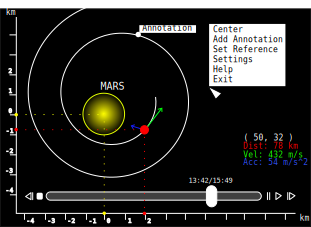
\includegraphics[width=1\textwidth]{mockup}
\caption{Mock-up of the Interface}
\label{fig:mockup}
\end{figure}

The design of the GUI (Graphical User Interface) is minimalistic. It is meant to be able to fulfil all the required features mentioned before in a comfortable and simple way. By avoiding unneeded options and features, the window is much cleaner and the interface much more simple. This allows it to be comfortable for users of all levels.

In figure \ref{fig:mockup} you can see all the features. There are rulers indicating position relative to the current reference (in this case the reference is Mars). The current position and the current reference are both marked on the rules to make it easier to see. The trajectory is clearly visible for past and future positions and the acceleration and velocity vectors are drawn on the current position. On the bottom there is the time slider, which allows the user to play the entire animation or jump to a specific point in time. It fades out when not being used until the mouse is over it again.

On the right there is both the current position (relative to reference). Below it is the distance from the reference, the current velocity and the current acceleration in numerical values. These can be hidden or be changed to use other units by the settings tab in the menu. To open the menu you just have to right click as shown in figure \ref{fig:mockup}. As you can see there's few items to try to keep the interface simple. The most important being the ability to add annotations, change references and change settings. You can see an annotation on the trajectory in the figure also.

The mock-up is just for reference. The final application will most likely not look like the mock-up but will look similar. 


\section{Interface}

The human interface will consist of two parts. First the user will be able to pass command line arguments to the application, allowing him to configure core settings which can also be saved in a configuration file. This allows scripted settings to be done.

The second and more important interface is the active interface when a trajectory is being visualized. This interface consists of interpreting user input that can come from the mouse or the keyboard to manipulate the visualization. The interface is to be simple and intuitive. This means it should follow the movements of other CAD applications. The more intuitive the interface is, the smaller the learning curve will be for the users. To make the application even more intuitive it should use the context for each input. For example double clicking an object could set it as a reference.

Some of the common mouse functionality is:
\begin{itemize}
\item Rotation with the middle mouse button
\item Zooming with mouse scrolling
\item Shift and drag moves around the plane perpendicular to the camera
\item Clicking selects object
\item Right clicking opens context sensitive menu
\item Double clicking does context sensitive action
\end{itemize}

Some of the common keyboard functionality is:
\begin{itemize}
\item Numpad to move the camera around
\item Hotkeys to different actions to avoid mouse usage for power users
\end{itemize}

The trajectory visualizer will follow the common functionality to simplify the experience for new users.


\section{Conclusions}

There is much more to application design than expected when it comes to ergonomics and intuitiveness. These aspects are often overlooked and can bring problems when the application is finished and no one is able to use it well. By thinking about these aspects before the start of a project, one can already predict where conflicts are most likely to occur and how to avoid them. This is one of the best ways to ensure the quality of the final product like in this case the 3D Visualization for Interplanetary Trajectories.


\end{document}

